\section{Elecci'on de Coordinador en un Sistema Distribuido con \emph{Token Ring}}
En este simulador intentamos mostrar c'omo es llevada acabo la elecci'on de un
nuevo coordinador mediante \emph{token ring} ante la caida del coordinador de
un sistema distribuido se cae por alg'un motivo.

Decidimos suponer una red de ocho computadoras interconectadas que tienen como
coordinador al nodo de mayor n'umero que esta activo. Creemos que ocho
computadoras es un n'umero suficiente para ilustrar el algoritmo sin p'erdida
de generalidad.

La simulaci'on permite poner \emph{online/offline} los distintos nodos de la
red y a los activos les permite verificar que el coordinador est'e vivo. Esto
se hace enviando un mensaje AYA (\emph{Are you alive}), mensaje que en el
coordinador deber'ia responder con un IAA (\emph{I am alive}).

Cuando un nodo detecta que el coordinador actual no est'a vivo, dado que no
respondio el AYA que le envi'o (ocurre un  \emph{timeout} en la espera de la
respusta), arma un mensaje que contendrá una lista en la cual se ir'an anotando
los nodos activos. Inicialmente se incluye a si mismo en
esta lista y la envia a trav'es de la red a la siguiente computadora
(recordemos que cada computadora tiene un n'umero con el que definimos cu'al es
la pr'oxima). Si este nodo esta activo, recibe el mensaje, se agrega a la lista
y repite el procedimiento con su sucesor. En caso contrario el nodo emisor le 
envia el mensaje con la lista de nodos a la siguiente computadora repiti'endose
el proceso anterior (si est'a activo se agrega y sino se reenv'ia \ldots). Una vez
que la lista viaja por toda la red dando una vuelta entera al anillo vuelve al
nodo emisor, este inspecciona la lista para elegir al nuevo coordinador. El
nodo que reemplazar'a al coordinador caido es el que tenga el n'umero m'as
grande de la lista. El nodo que comenzo el proceso de selecci'on avisa al resto
de los nodos que el nuevo coordinar ha sido elegido y avisa el n'umero del
mismo.

%Vale aclarar que si bien en este ejemplo el 'unico nodo caido es el
%coordinador, podr'ia pasar que otro nodo este caido tambi'en, en este caso
%cuando el mensaje se envie al nodo caido y no conteste entonces el mensaje
%ser'a enviado nuevamente al siguiente nodo, de la misma forma que se hace
%cuando el mensaje es enviado al coordinador cuando este esta caido. Adem'as si
%un nodo envia un AYA en un instante en el que el coordinador esta activo, este
%contestar'a inmediatamente y no ser'a necesario ning'un algoritmo de
%selecci'on.

\newpage
\subsection{Ejemplo de funcionamiento}
Veamos ahora un ejemplo de ejecuci'on del simulador:

Supongamos que tenemos una red de ocho computadoras numeradas del cero al
siete. El nodo siete es el coordinador, pero por alguna raz'on deja de
responder y el nodo n'umero tres realiza un AYA al nodo coordinador para saber
si esta activo, al no responder luego de un lapso de tiempo se produce un
\emph{timeout} y  nodo n'umero tres arma la lista de nodos activos, se incluye
en esta y la env'ia al siguiente nodo, en este caso ser'a el numero cuatro, que
se incluir'a y asi sucesivamente hasta llegar al n'umero 6. En este caso el
nodo n'umero 6 no recibe respuesta del nodo n'umero siete y entonces lo saltea,
envi'andole la lista al n'umero cero, siguiendo este esquema la lista llegar'a
nuevamente al n'umero tres, que es el que inici'o el proceso de elecci'on con
lo cual sabr'a que debe realizar la selecci'on del nuevo coordinador entre los
nodos que figuran en el mensaje. Para esto toma el mayor valor de la lista,
resultando este el n'umero seis y le envia un mensaje al nodo n'umero seis para
que comience a coordinar a la red.


\begin{figure}[h!]
\centering
 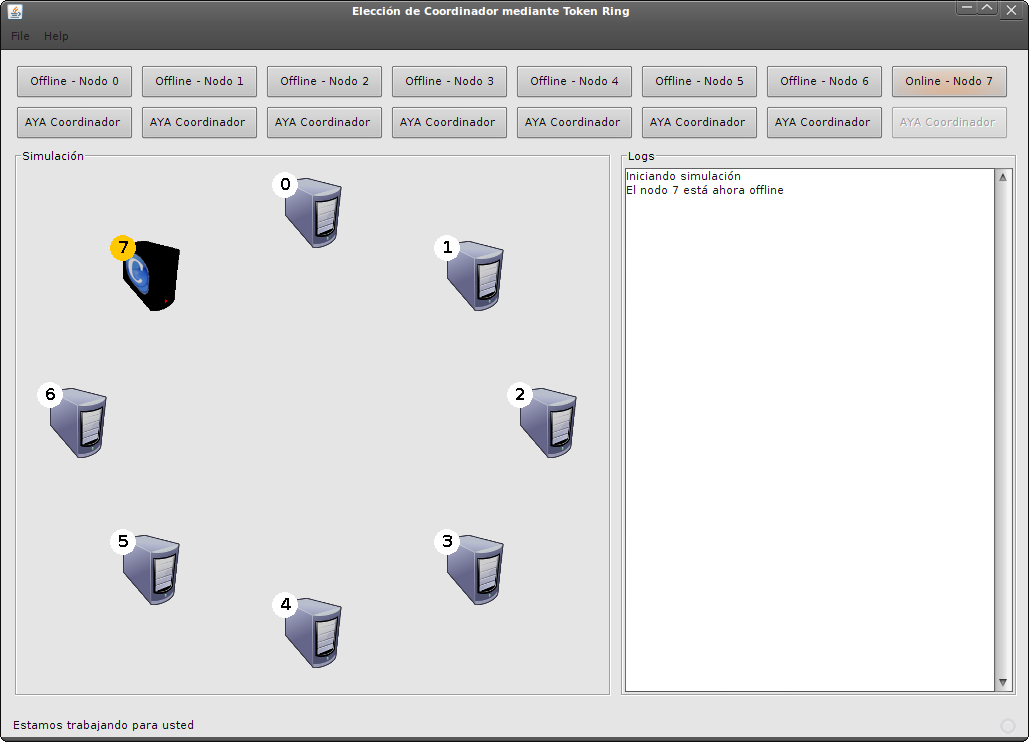
\includegraphics[scale=0.33,keepaspectratio=true]{./imagenes/tokenRing/token1.png}
 \caption{Aqu'i vemos al simulador con el nodo siete caido.}
\end{figure}
\newpage
\begin{figure}[h!]
\centering
 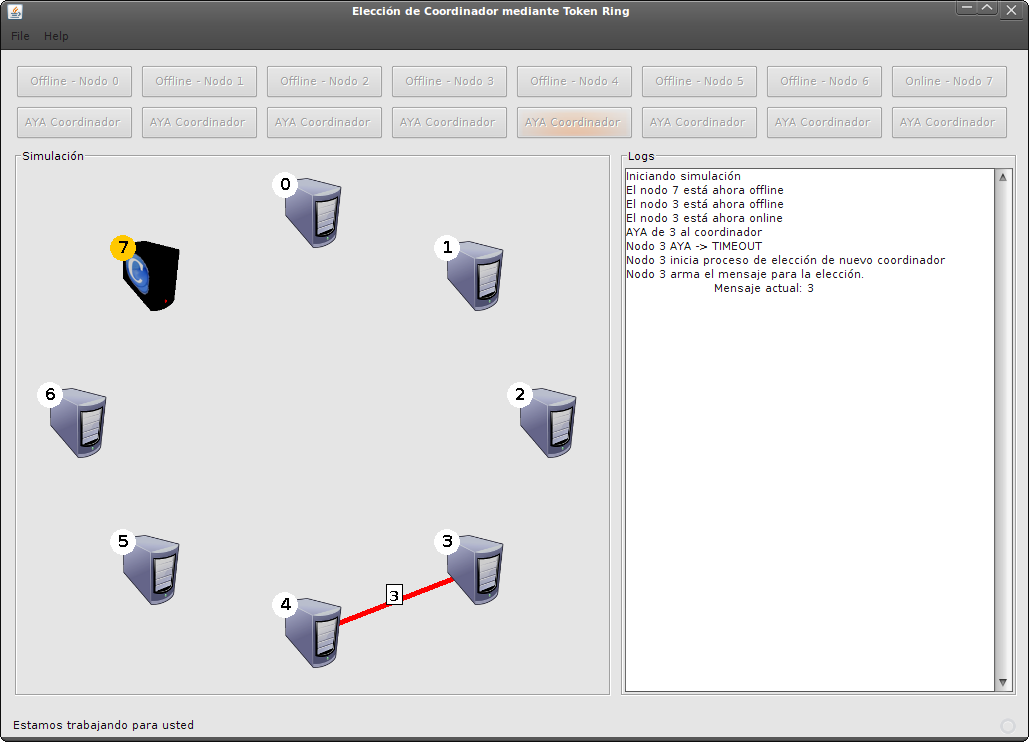
\includegraphics[scale=0.33,keepaspectratio=true]{./imagenes/tokenRing/token2.png}
 \caption{El nodo tres no recibe respuesta del coordinador y comienza el proceso de elecci'on.}
\end{figure}

\begin{figure}[h!]
\centering
 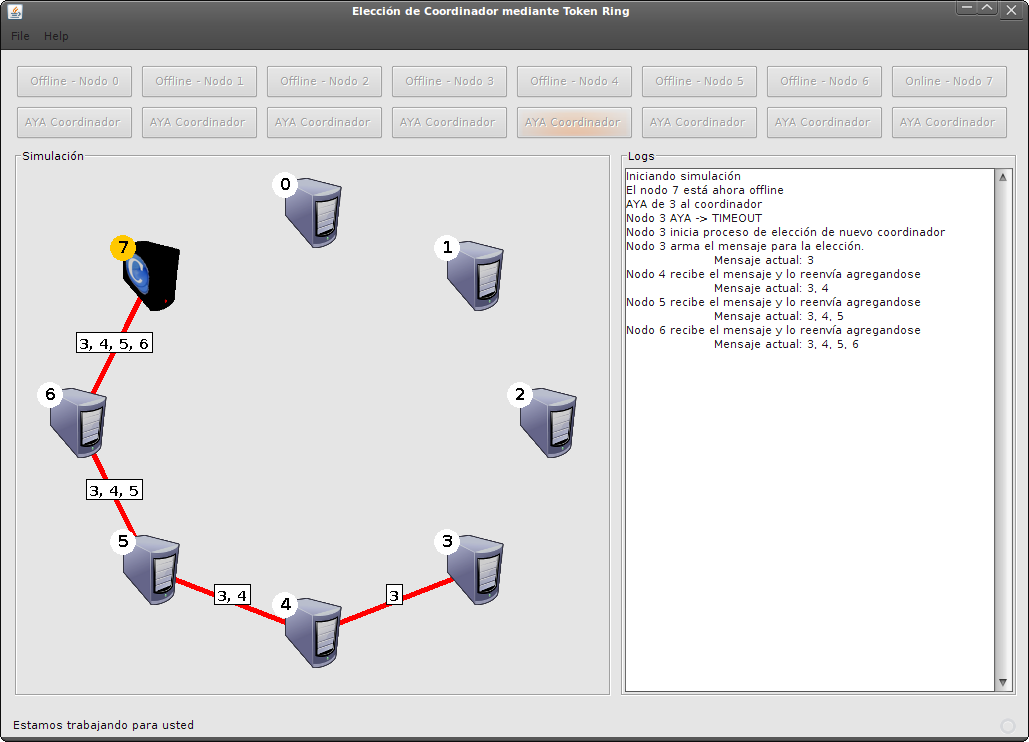
\includegraphics[scale=0.33,keepaspectratio=true]{./imagenes/tokenRing/token3.png}
 \caption{El nodo seis envia el mensaje al nodo siete.}
\end{figure}

\newpage
\begin{figure}[h!]
\centering
 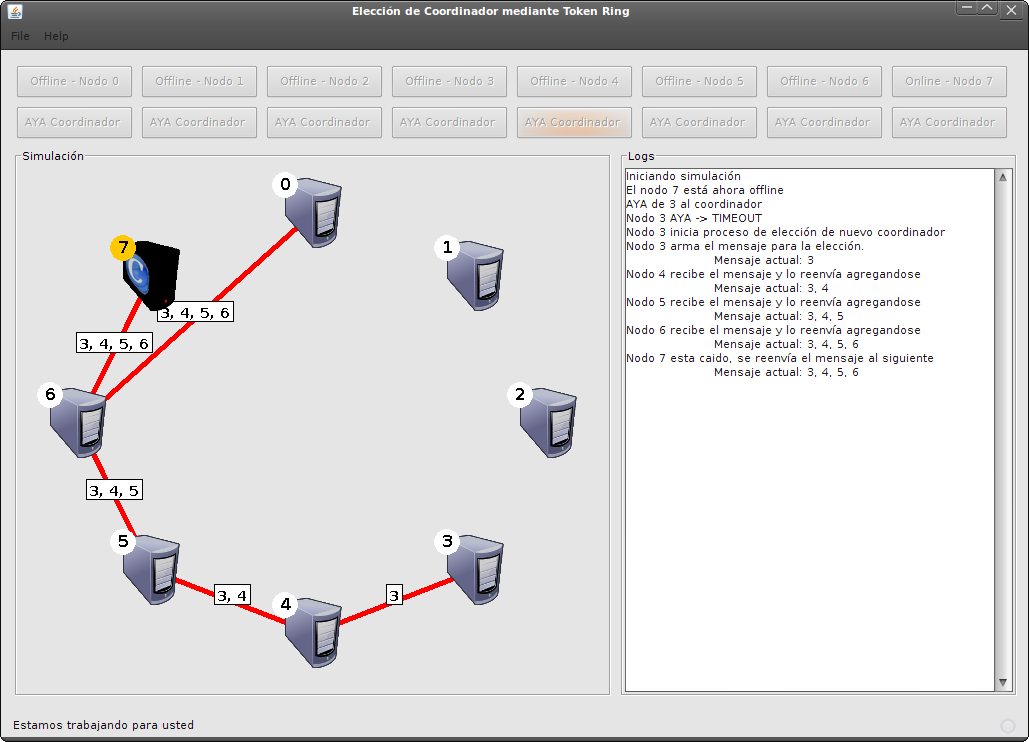
\includegraphics[scale=0.33,keepaspectratio=true]{./imagenes/tokenRing/token4.png}
 \caption{Ocurre el \emph{timeout} en la espera de la confirmaci'on de
recepci'on por parte del nodo siete. El nodo 6 env'ia el mensaje al nodo cero.}
\end{figure}

\begin{figure}[h!]
\centering
 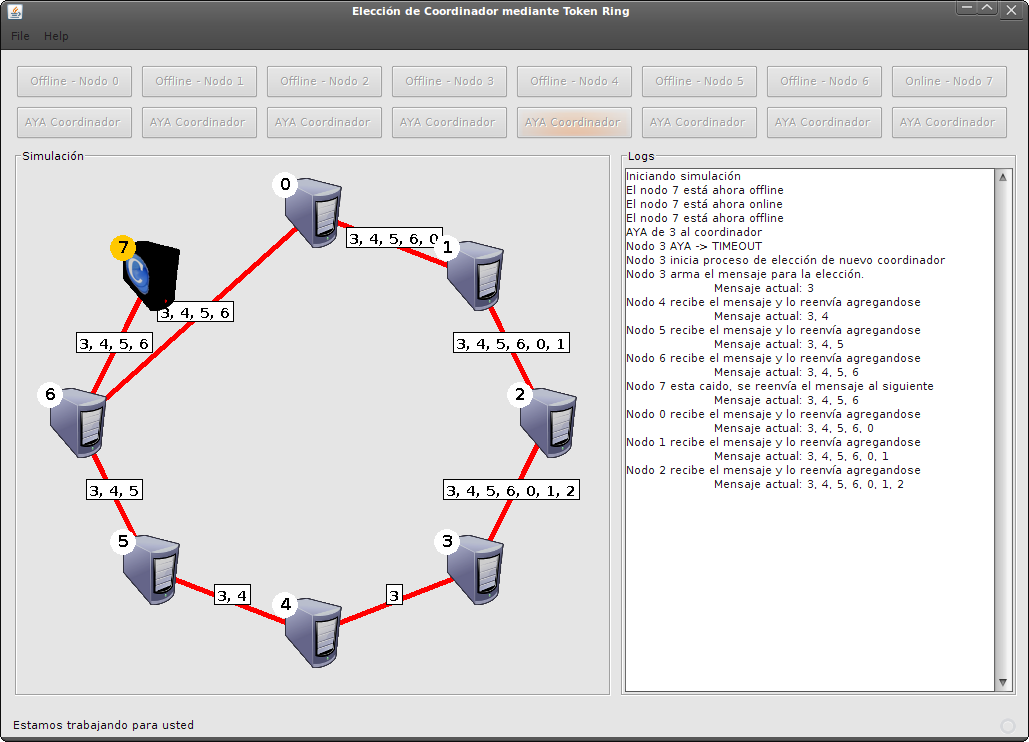
\includegraphics[scale=0.33,keepaspectratio=true]{./imagenes/tokenRing/token5.png}
 \caption{El mensaje termina de pasar por todos los nodos y el nodo tres, selecciona el mayor de los n'umeros en la lista.}
\end{figure}
\newpage

\begin{figure}[h!]
\centering
 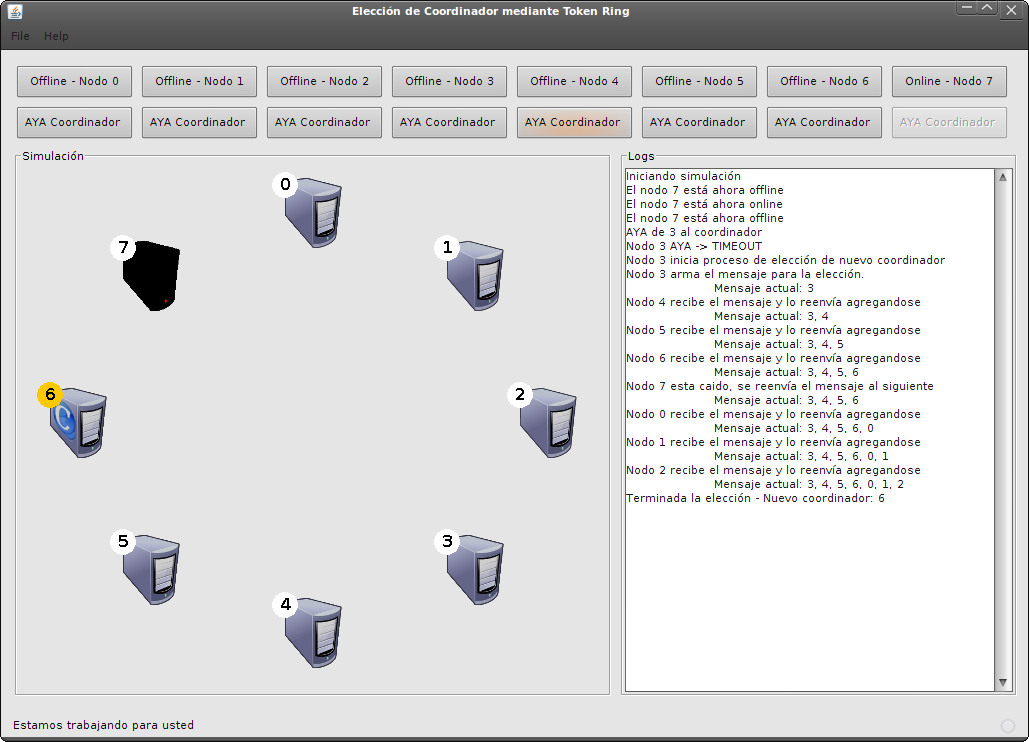
\includegraphics[scale=0.33,keepaspectratio=true]{./imagenes/tokenRing/token6.png}
 \caption{El nodo n'umero tres avisa al resto que el nuevo coordinador es el n'umero seis, este comienza a coordinar al todo el sistema.}
\end{figure}

\subsubsection*{Otro ejemplo}
Veamos un caso en el que m'as de un nodo no responde a los pedidos de los dem'as.

\begin{figure}[h!]
\centering
 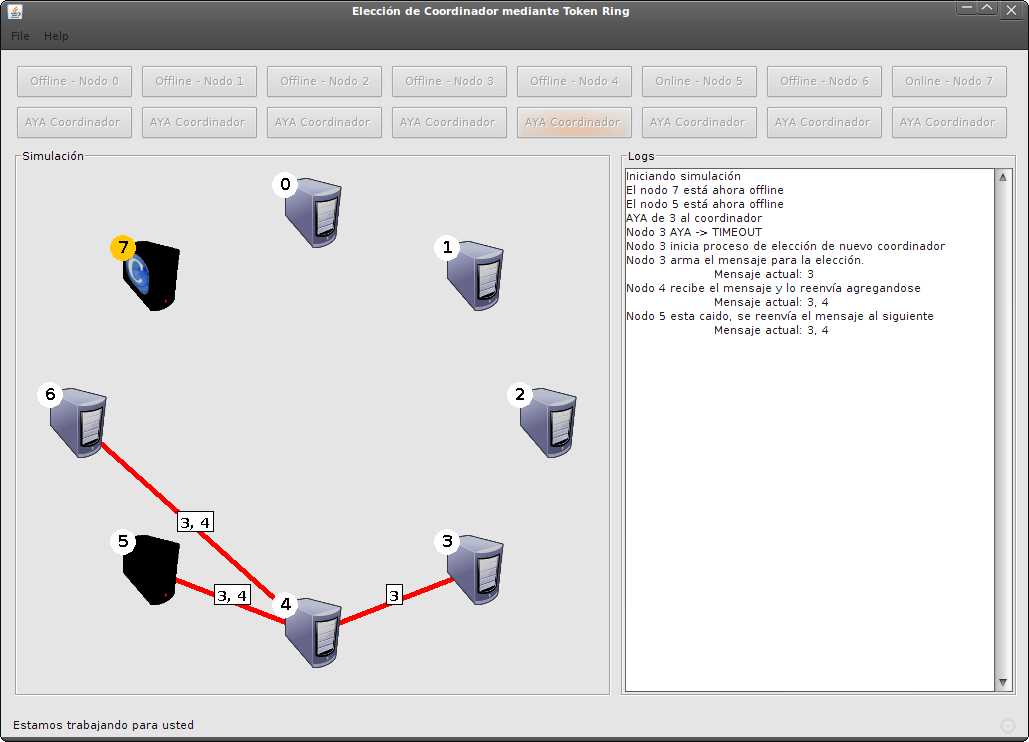
\includegraphics[scale=0.33,keepaspectratio=true]{./imagenes/tokenRing/token7.png}
 \caption{En este caso el nodo siete y el nodo cinco estan caidos, podemos observar como el nodo cuatro envia la lista al nodo seis al determinar que el cinco esta caido.}
\end{figure}
\newpage

\begin{figure}[h!]
\centering
 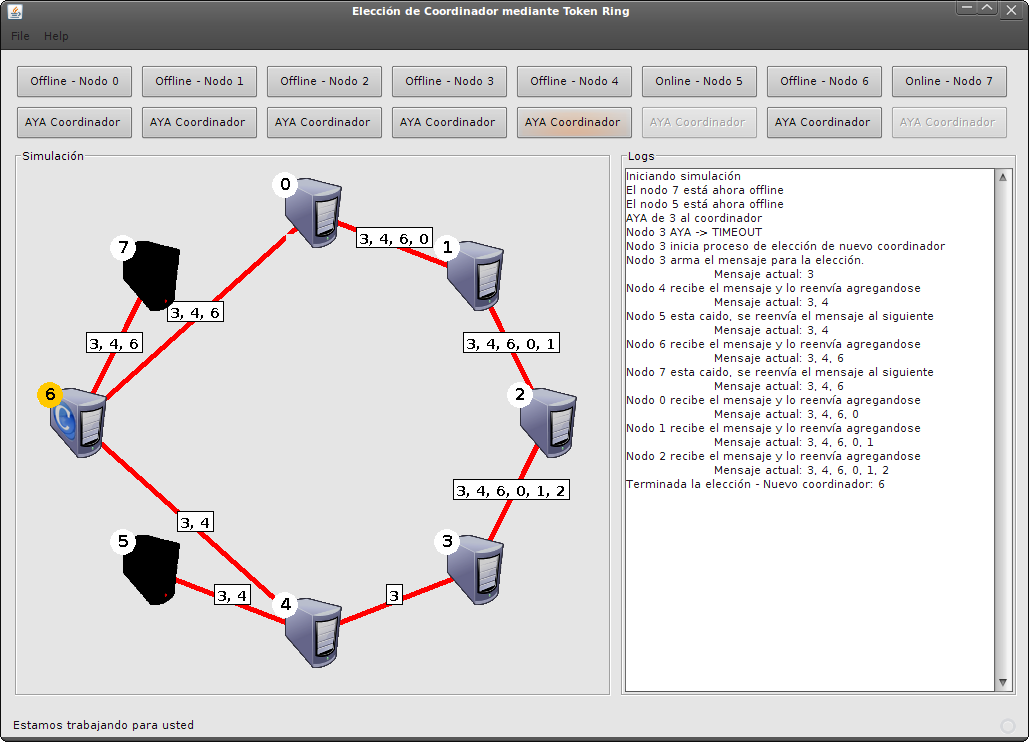
\includegraphics[scale=0.33,keepaspectratio=true]{./imagenes/tokenRing/token8.png}
 \caption{Terminada la elecci'on del nuevo coordinador, podemos observar como el mensaje paso por todos los nodos activos y el nodo seis es el coordinador.}
\end{figure}

